\section{Une éolienne dans le jardin}\label{ex:eolienne}
	
Julie a installé une éolienne dans son jardin pour son éclairage extérieur. On a symbolisé le fonctionnement de l'éolienne par une chaîne énergétique.

\begin{center}
	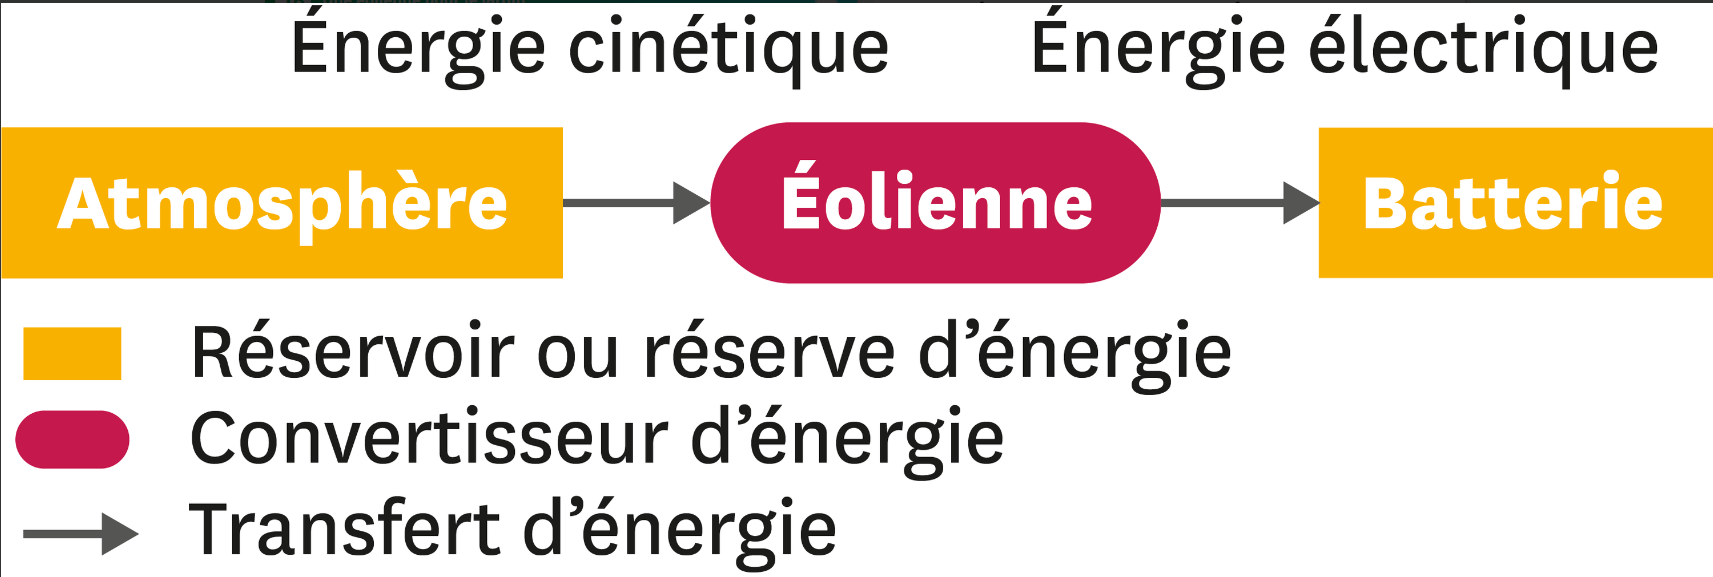
\includegraphics[scale=0.2]{img/chaine}
\end{center}

\begin{questions}
	\question Quel est le réservoir d'énergie qui transmet de l'énergie à l'éolienne ?
		\begin{solution}
			Le réservoir qui transmet de l'énergie à l'éolienne est l'atmosphère.
		\end{solution}
	
	\question Quelle forme d'énergie est transmise à l'éolienne ?
		\begin{solution}
			La forme d'énergie transmise à l'éolienne est de l'énergie cinétique.
		\end{solution}
	
	
	\question Quel est le réservoir d'énergie qui reçoit de l'énergie de la part de l'éolienne ?
		\begin{solution}
			Le réservoir qui reçoit de l'énergie de la part de l'éolienne est la batterie.
		\end{solution}
	
	\question Sous quelle forme se fait le transfert d'énergie de l'éolienne vers le réservoir final ?
		\begin{solution}
			Le transfert d'énergie vers le réservoir final se fait sous forme d'énergie électrique.
		\end{solution}
\end{questions}